\documentclass[11pt,a4paper]{article}

\usepackage[polish]{babel}
\usepackage[utf8]{inputenc}
\usepackage{polski}
\usepackage[T1]{fontenc}
\usepackage{indentfirst}
\usepackage{wrapfig}    % for wrapping figures, tables
\usepackage{isotope}
\usepackage{hyperref}
\usepackage{amsmath}
\usepackage{amssymb}
\usepackage{bm}
\usepackage{gensymb}
\usepackage{epsfig}
\usepackage{graphics}
\usepackage[shortlabels]{enumitem}
\usepackage{xspace}
\xspaceaddexceptions{[]\{\}}

%\def\hidesolutions{}  %← show solutions. Comment out to show solutions

%
%
%fixpagesize
\pagestyle{empty}
\addtolength{\textwidth}{4cm}
\addtolength{\textheight}{6cm}
\addtolength{\evensidemargin}{-3cm}
\addtolength{\oddsidemargin}{-2cm}
\addtolength{\topmargin}{-3cm}
\parindent=0cm

%
%
% Changes figure placing algorithm
\renewcommand{\topfraction}{1}       % maximal fraction of a page allowed for figures
\renewcommand{\textfraction}{0.15}   % minimal number of text for figure-text shared pages
\renewcommand{\floatpagefraction}{0.95} % if two above does not help, this could do the job 
                                        % must be: floatpagefraction < topfraction !!!!
\renewcommand{\textfraction}{0} % minimum fraction of page, which must be  devoted to text
\renewcommand{\topfraction}{1}  % maximum fraction at top, which can be occupied whit floats
\setcounter{totalnumber}{400}   % increase the number of floats for one page
\setcounter{topnumber}{200}     % at all/top/bottom.
\setcounter{bottomnumber}{200}  %

%
%
%small distance in list/item/enum for enumitem package
\setlist[itemize,enumerate]{topsep=0em}
\setlist{noitemsep}

%Nuclear notations: usage \nucl{235}{92}{U}. Math mode optional
\newcommand{\nucl}[3]{\ensuremath{
  \phantom{\ensuremath{^{#1}_{#2}}}
  \llap{\ensuremath{^{#1}}}
  \llap{\ensuremath{_{\rule{0pt}{.75em}#2}}}
  \mbox{#3} } 
} 

\newcounter{zadanie}\newcommand{\zadanie}[1][]{\addtocounter{zadanie}{1} ~\\  {\bf \emph{Exercise \arabic{zadanie} #1 }} \\}
\newcounter{zaddom}\newcommand{\zaddom}[1][]{\addtocounter{zaddom}{1} ~\\  {\bf \emph{Homework \arabic{zaddom} #1 }} \\}

%dynamic solutions hiding
\usepackage{comment}

\newif\ifhidesolutions
\ifdefined\hidesolutions
  \hidesolutionstrue
\else
  \hidesolutionsfalse
\fi

\ifhidesolutions
  \excludecomment{solution}
\else
  \newenvironment{solution}{\vspace{1cm} \par\textbf{Solution.} \vspace{1cm}}{\newpage}
\fi
%%%%%%%%%%%%%%%%%%%%%%%%%%%%%%%%%%%%%%%%%%
\begin{document}         

%%%%%%%%%%%%%%%%%%%%%%%%%%%%%%%%%%%%%%%%%%%%%%%%%%%%%
\begin{centering}
  {\bf {\Large
 Introduction to Experimental Particle Physics I \\
  Set V: Interactions.
  }} \\  
\end{centering}

\vspace{1cm}
%%%%%%%%%%%%%%%%%%%%%%%%%%%%%%%%%%%%%%%%%%%%%%%%%%%%%%%
\zadanie[Mandelstam variables]

Consider $2\to2$ scattering in three configurations, usually denoted as 
s-channel, t-channel and u-channel. Write out formula for $q^{2}$ of the 
mediator, and calculate their sum: $q_{s}^{2}+q_{t}^{2}+q_{u}^{2}$.

%add picture
\begin{center}
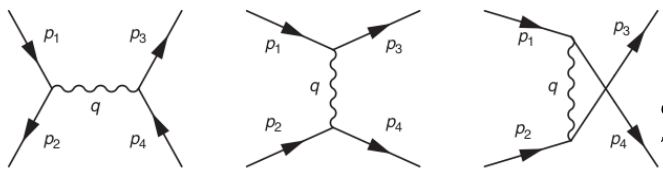
\includegraphics[width=0.6\textwidth]{s_t_u_diagrams.png}
\end{center}

{\bf Hint:} Use the four-momentum conservation.

\begin{solution}

Mandelstam variables are defined as follows:
\begin{align*}
  q_s^2 &= (p_1 + p_2)^2 = (p_3 + p_4)^{2} \\
  q_t^2 &= (p_1 - p_3)^2 = (p_2 - p_4)^2 \\
  q_u^2 &= (p_1 - p_4)^2 = (p_2 - p_3)^2 \\
\end{align*}

The sum:
\begin{align*}
  (q_s^2 + q_t^2 + q_u^2) =& (p_1 + p_2)^2 + (p_1 - p_3)^2 + (p_1 - p_4)^2 = \\
  =& p_1^2 + p_2^2 + 2p_1\cdot p_2 + p_1^2 + p_3^2 - 2p_1\cdot p_3 + p_1^2 + p_4^2 - 2p_1\cdot p_4 = \\
  =& 3p_1^2 + p_2^2 + p_3^2 + p_4^2 + 2p_1\cdot p_2 - 2p_1\cdot p_3 - 2p_1\cdot p_4 = \\
  =& 3p_1^2 + p_2^2 + p_3^2 + p_4^2 + 2p_1\cdot (p_2 - p_3 - p_4) = \\
  & || p_{1} + p_2 = p_3 + p_4 \Rightarrow p_2 - p_3 - p_4 = -p_1 || \\
  =& 3p_1^2 + p_2^2 + p_3^2 + p_4^2 - 2p_1^2 = p_1^2 + p_2^2 + p_3^2 + p_4^2 = \\
  & m_{1}^2 + m_2^2 + m_3^2 + m_4^2
\end{align*}


\end{solution}
%%%%%%%%%%%%%%%%%%%%%%%%%%%%%%%%%%%%%%%%%%%%%%%%%%%%%%%
%%%%%%%%%%%%%%%%%%%%%%%%%%%%%%%%%%%%%%%%%%%%%%%%%%%%%%%
\zadanie[Perurbative series]

Consider quantum harmonic oscillator with the Hamiltonian:
\begin{align*}
  H = \frac{p^2}{2m} + \frac{1}{2} m \omega^2 x^2 + \lambda x^4
\end{align*}
where $\lambda$ is a small parameter. 
Using perturbation theory, calculate the first order wave function correction 
for the ground state. \\

{\bf Hint:} The only non-zero matrix elements of $\langle n|\hat{x}^4|0\rangle$ are:
\begin{align*}
   \langle 0 | \hat{x}^4 | 0 \rangle =& \frac{3}{4} \alpha^{4} \\
   \langle 2 | \hat{x}^4 | 0 \rangle =& \frac{3}{2} \alpha^{4} \\
   \langle 4 | \hat{x}^4 | 0 \rangle =& \frac{\sqrt{6}}{2} \alpha^{4} \qquad \text{where } \alpha = \sqrt{\frac{\hbar}{m \omega}} 
\end{align*}


\begin{solution}

Wave function correction is given by the formula:
\begin{align*}
  |\psi_0^{(1)}\rangle = \sum_{n\neq 0} \frac{\langle n | \hat{H}' | 0 \rangle}{E_0 - E_n} |n\rangle
\end{align*}
where $\hat{H}' = \lambda x^4$ is the perturbation. The only non-zero matrix elements are for $n=2$ and $n=4$, so we have:
\begin{align*}
  |\psi_0^{(1)}\rangle = \frac{\langle 2 | \lambda x^4 | 0 \rangle}{E_0 - E_2} |2\rangle + \frac{\langle 4 | \lambda x^4 | 0 \rangle}{E_0 - E_4} |4\rangle
\end{align*}
The energy levels of the harmonic oscillator are given by $E_n = \hbar \omega (n + \frac{1}{2})$, so we have:
\begin{align*}
  E_0 - E_2 = \hbar \omega (0 + \frac{1}{2}) - \hbar \omega (2 + \frac{1}{2}) = -2\hbar \omega \\
  E_0 - E_4 = \hbar \omega (0 + \frac{1}{2}) - \hbar \omega (4 + \frac{1}{2}) = -4\hbar \omega    
\end{align*}
Substituting the matrix elements and energy differences, we get:
\begin{align*}
  |\psi_0^{(1)}\rangle = -\frac{\lambda \alpha^{4}}{2\hbar \omega} \left[\frac{3}{2} |2\rangle + \frac{\sqrt{6}}{2} |4\rangle  \right] = \\
  = -\frac{\lambda \hbar}{2 m^{2} \omega^{3}} \left[\frac{3}{2} |2\rangle + \frac{\sqrt{6}}{2} |4\rangle  \right] = \\
\end{align*}  

The wave function to first order is then:
\begin{align*}
  |\psi_0\rangle = |0\rangle + |\psi_0^{(1)}\rangle = |0\rangle -\frac{\lambda \hbar}{2 m^{2} \omega^{3}} \left[\frac{3}{2} |2\rangle + \frac{\sqrt{6}}{2} |4\rangle  \right]
\end{align*}


\end{solution}

%%%%%%%%%%%%%%%%%%%%%%%%%%%%%%%%%%%%%%%%%%%%%%%%%%%%%%%
%%%%%%%%%%%%%%%%%%%%%%%%%%%%%%%%%%%%%%%%%%%%%%%%%%%%%%%
\end{document}
